%+210 to left and -210 to right if I want to move one subfigure.

\begin{figure}[!h]
%\vspace{-1pt} %takes away some white space before figure
\centering
\begin{subfigure}[b]{0.5\textwidth}
\centering
	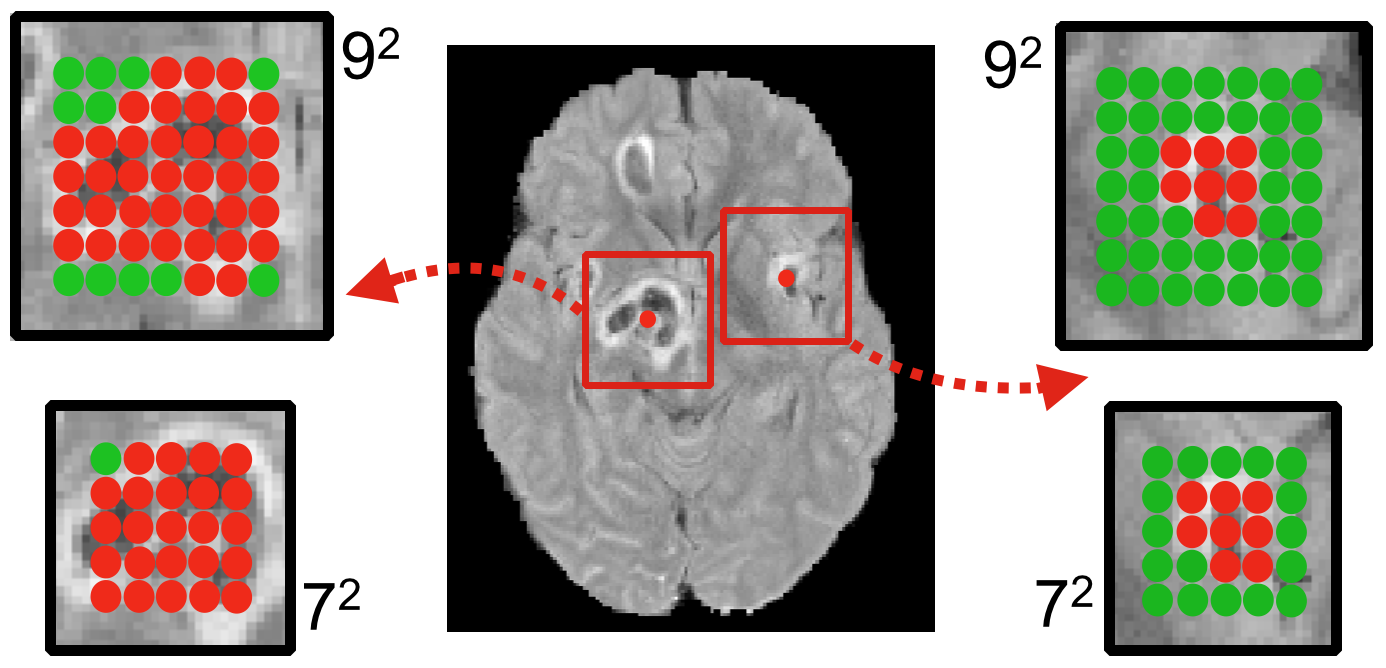
\includegraphics[clip=true, trim=0pt 0pt 0pt 0pt, width=1.0\textwidth]{figures/methodSection/denseTraining/segmentsVisual.png}
\end{subfigure}

\caption{Consider a network with a 2D receptive field of $3^2$ (for illustration) densely-applied on the depicted lesion-centred image segments of size $7^2$ or $9^2$. Relatively more background (green) is captured by larger segments and around smaller lesions.}
\label{fig:segmentsVisual}
\end{figure}